\documentclass{article}

\usepackage{arxiv}

\usepackage[utf8]{inputenc} % allow utf-8 input
\usepackage[T1]{fontenc}    % use 8-bit T1 fonts
\usepackage{lmodern}        % https://github.com/rstudio/rticles/issues/343
\usepackage{hyperref}       % hyperlinks
\usepackage{url}            % simple URL typesetting
\usepackage{booktabs}       % professional-quality tables
\usepackage{amsfonts}       % blackboard math symbols
\usepackage{nicefrac}       % compact symbols for 1/2, etc.
\usepackage{microtype}      % microtypography
\usepackage{graphicx}

\title{Neo Cocoon: Low-cost and Portable Neonatal Protection and
Development System}

\author{
    Karthik M Dani
   \\
    Dept of Medical Electronics Engineering \\
    B.M.S College of Engineering \\
  Bangalore - 560019 \\
  \texttt{\href{mailto:karthik.ml22@bmsce.ac.in}{\nolinkurl{karthik.ml22@bmsce.ac.in}}} \\
   \And
    Sanjana WG
   \\
    Dept of Medical Electronics Engineering \\
    B.M.S College of Engineering \\
  Bangalore - 560019 \\
  \texttt{\href{mailto:sanjana.ml22@bmsce.ac.in}{\nolinkurl{sanjana.ml22@bmsce.ac.in}}} \\
   \And
    Darshan S K
   \\
    Dept of Medical Electronics Engineering \\
    B.M.S College of Engineering \\
  Bangalore - 560019 \\
  \texttt{\href{mailto:darshan.ml22@bmsce.ac.in}{\nolinkurl{darshan.ml22@bmsce.ac.in}}} \\
   \And
    Dr.~H. N. Suma
   \\
    Dean Innovation \\
    B.M.S College of Engineering \\
  Bangalore - 560019 \\
  \texttt{\href{mailto:hns.ml@bmsce.ac.in}{\nolinkurl{hns.ml@bmsce.ac.in}}} \\
   \And
    Mr.~Balaji Raghavendra S
   \\
    Founder and CEO \\
    Piroya Technologies \\
  Bangalore - 560019 \\
  \texttt{\href{mailto:balaji.s@piroya.com}{\nolinkurl{balaji.s@piroya.com}}} \\
  }


% tightlist command for lists without linebreak
\providecommand{\tightlist}{%
  \setlength{\itemsep}{0pt}\setlength{\parskip}{0pt}}


% Pandoc citation processing
%From Pandoc 3.1.8
% definitions for citeproc citations
\NewDocumentCommand\citeproctext{}{}
\NewDocumentCommand\citeproc{mm}{%
  \begingroup\def\citeproctext{#2}\cite{#1}\endgroup}
\makeatletter
 % allow citations to break across lines
 \let\@cite@ofmt\@firstofone
 % avoid brackets around text for \cite:
 \def\@biblabel#1{}
 \def\@cite#1#2{{#1\if@tempswa , #2\fi}}
\makeatother
\newlength{\cslhangindent}
\setlength{\cslhangindent}{1.5em}
\newlength{\csllabelwidth}
\setlength{\csllabelwidth}{3em}
\newenvironment{CSLReferences}[2] % #1 hanging-indent, #2 entry-spacing
 {\begin{list}{}{%
  \setlength{\itemindent}{0pt}
  \setlength{\leftmargin}{0pt}
  \setlength{\parsep}{0pt}
  % turn on hanging indent if param 1 is 1
  \ifodd #1
   \setlength{\leftmargin}{\cslhangindent}
   \setlength{\itemindent}{-1\cslhangindent}
  \fi
  % set entry spacing
  \setlength{\itemsep}{#2\baselineskip}}}
 {\end{list}}
\usepackage{calc}
\newcommand{\CSLBlock}[1]{#1\hfill\break}
\newcommand{\CSLLeftMargin}[1]{\parbox[t]{\csllabelwidth}{#1}}
\newcommand{\CSLRightInline}[1]{\parbox[t]{\linewidth - \csllabelwidth}{#1}\break}
\newcommand{\CSLIndent}[1]{\hspace{\cslhangindent}#1}

\begin{document}
\maketitle


\begin{abstract}
This project addresses the critical issue of neonatal care by aiming to
develop an affordable medical device, particularly focusing on the high
rates of morbidity and mortality among preterm infants. In 2020,
approximately 13.4 million premature births occurred globally, with a
significant number resulting in complications that lead to infant
mortality, particularly in low-income countries. By leveraging
non-invasive technologies for monitoring vitals of neonates, this
project aims to enhance the detection and management of neonatal
jaundice and hypothermia---two prevalent conditions affecting newborns.

The study utilizes a combination of non contact infrared thermometry,
phototherapy techniques, Internet of Medical Things (IoMT) and efficient
RDMS, from monitoring body temperature, detecting and treating jaundice,
sharing it to the device hosted webserver for ease of use and access.
The effectiveness of these interventions will be evaluated through a
systematic workflow that integrates data collection, processing, and
real-time monitoring. Additionally, the project emphasizes the
importance of immediate postnatal care practices, such as drying and
wrapping newborns, to mitigate hypothermia risk and improve thermal
protection.

Through this multidisciplinary approach, the project aspires to develop
cost-effective solutions that can be implemented in resource-limited
settings, thereby reducing neonatal mortality rates. The anticipated
outcomes include improved clinical practices and increased accessibility
to essential neonatal care technologies, ultimately contributing to
better health outcomes for vulnerable population.
\end{abstract}

\keywords{
    NICU
   \and
    Medical Device
   \and
    IoMT
   \and
    AI
   \and
    Neonatal Protection
   \and
    Portable
   \and
    Monitoring
   \and
    Premature Infants
   \and
    Temperature
   \and
    SpO2
   \and
    Heart Rate
   \and
    ECG
   \and
    Phototherapy
   \and
    Data Logging
   \and
    User-Friendly Interface
   \and
    Microprocessor
   \and
    Microcontroller
   \and
    Healthcare
   \and
    Jaundice Treatment
  }

\section{Introduction}\label{introduction}

Babies born before the completion of 37 weeks of pregnancy are
classified as premature {[}1{]}. They are further categorized as
follows:

\begin{enumerate}
\def\labelenumi{\arabic{enumi}.}
\item
  \textbf{Extremely premature:} Less than 28 weeks
\item
  \textbf{Very premature:} 28 to 32 weeks
\item
  \textbf{Moderate to late premature:} 32 to 37 weeks
\end{enumerate}

\subsection{Background}\label{background}

\subsubsection{Low Birth Weight (LBW) as consequence of Pre Mature
Birth}\label{low-birth-weight-lbw-as-consequence-of-pre-mature-birth}

\textbf{Low Birth Weight (LBW)} refers to infants born weighing less
than 5 pounds, 8 ounces (2,500 grams). In contrast, the average newborn
typically weighs around 8 pounds. Much of a baby's weight is accumulated
in the final weeks of pregnancy, so being born prematurely often results
in low birth weight {[}2{]}.

Another cause of Low Birth weight is condition called
\textbf{Intrauterine Growth Restriction (IUGR)} arises when a baby does
not grow adequately during pregnancy.

\paragraph{Health Complications of Low Birth
Weight}\label{health-complications-of-low-birth-weight}

Infants with low birth weight encounter numerous health complications
that can adversely affect their growth and development. One of the
significant issues they face is reduced oxygen levels at birth, which
may lead to immediate respiratory difficulties. These infants often
struggle to maintain a stable body temperature, putting them at risk for
hypothermia. Additionally, many experience feeding challenges, as their
ability to suck may be compromised, resulting in inadequate weight gain.
Their underdeveloped immune systems make them more susceptible to
infections. Furthermore, low birth weight can lead to breathing issues
like infant respiratory distress syndrome, stemming from immature lung
development. Neurological problems may also arise, such as
intraventricular hemorrhage, which involves bleeding within the brain.
The risk of digestive complications, particularly necrotizing
enterocolitis, poses further concerns. Lastly, there is an elevated risk
of sudden infant death syndrome (SIDS) during the early months of life,
adding to the vulnerabilities faced by these infants. {[}2{]}

\paragraph{3 methods to address Low Birth Weight as a Medical
Electronics
Engineer}\label{methods-to-address-low-birth-weight-as-a-medical-electronics-engineer}

Management for LBW often involves:

\begin{enumerate}
\def\labelenumi{\arabic{enumi}.}
\item
  Care in a neonatal intensive care unit (NICU).
\item
  Temperature-controlled environments such as a warmer or an infant
  incubator.
\item
  Specialized feeding methods, including tube feeding for infants unable
  to suck, or intravenous (IV) feeding.
\end{enumerate}

While we choose the 2nd method to address the problem, we choose
innovation in domain of incubators instead of warmers for the reasons
listed in the latter sections.

\section{Motivation}\label{motivation}

\subsection{Pre Mature Birth
Statistics}\label{pre-mature-birth-statistics}

In 2020, 10\% of all births worldwide, equating to approximately 13.4
million, were premature. In 2019, around 900,000 children died due to
complications arising from preterm birth. In low-income countries,
nearly half of the infants born at or before 32 weeks gestation (i.e.,
two months premature) do not survive due to a lack of effective and
affordable care {[}1{]} {[}3{]}. See figure \ref{fig:fig1}

Furthermore, more than 90\% of extremely preterm infants (born before 28
weeks) in low-income settings die within the first few days of life, in
stark contrast to less than 10\% in high-income countries. It is
estimated that three-quarters of these deaths could be averted with
existing, cost-effective interventions. The rate of premature births in
2020 varied from 4\% to 16\% {[}3{]}.

\begin{figure}
  \centering
  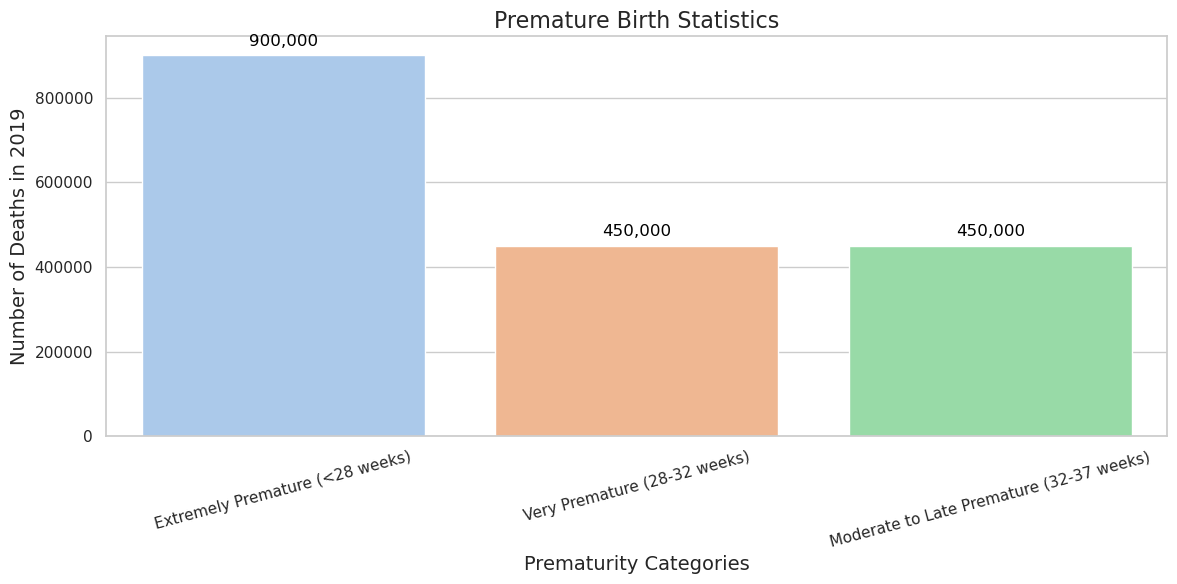
\includegraphics[width=350pt,height=200pt]{images/clipboard-1098342472.png} % Adjust the path to your image
  \caption{Global statistics on premature births in 2020, highlighting the prevalence of preterm births and associated mortality rates, particularly in low-income countries.}
  \label{fig:fig1}
\end{figure}

In 2022, nearly half (47\%) of all deaths among children under five
years old took place during the neonatal period, which refers to the
first 28 days of life. Every day, approximately 6,500 newborns die,
primarily due to inadequate quality of care at birth. Most neonatal
deaths (about 75\%) occur within the first week of life, highlighting
the urgent need for effective interventions during this crucial
timeframe. {[}4{]} See figure \ref{fig:fig2}

\begin{figure}
  \centering
  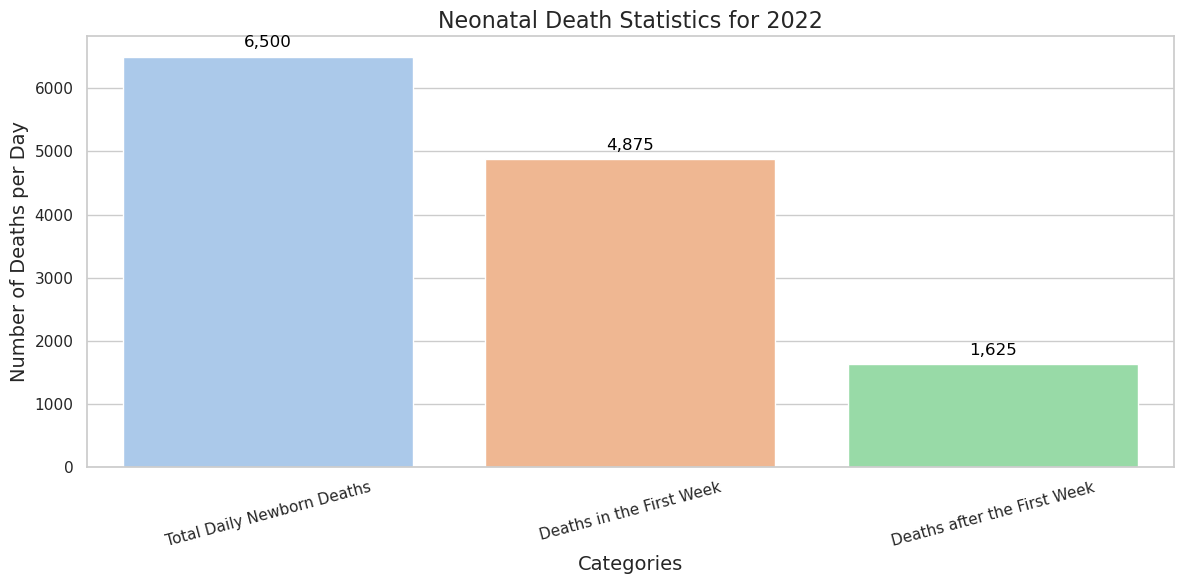
\includegraphics[width=350pt,height=200pt]{images/clipboard-3806704517.png} % Adjust the path to your image
  \caption{Nearly 47\% of child deaths under five occur in the neonatal period, underscoring the need for timely interventions.}
  \label{fig:fig2}
\end{figure}

Therefore the health outcomes for premature newborns in remote and
resource-limited areas stems from the critical need to address the
vulnerabilities these infants face. Premature babies are at a higher
risk of complications due to their underdeveloped physiological systems.
In regions where access to medical facilities and skilled healthcare
providers is limited, traditional neonatal care may not be feasible.
Thus, developing solutions that are smarter, safer, and responsive to
the unique challenges of these environments is essential. These
solutions should be designed to be user-friendly, minimizing the need
for extensive training and allowing caregivers to provide effective
support with limited resources. By focusing on reducing dependency on
human supervision, we can create reliable systems that ensure consistent
care for these vulnerable infants, ultimately aiming to improve their
survival rates and long-term health outcomes.

\section{Literature Survey}\label{literature-survey}

WHo claims Hypothermia is a significant contributor to neonatal illness
and death, particularly among low birth weight and normal newborns. To
combat this, thermal protection measures are crucial for maintaining a
normal body temperature of 36.5--37.5°C after birth, as newborns are
often exposed to cooler environments that cause rapid heat loss. {[}1{]}

\[
SizeOfInfant \propto T_{OutsideNormal}
\]

Where, \(T_{OutsideNormal}\) is the Temperature outside the normal
range.

This heat loss can occur through various mechanisms, including
evaporation, conduction, convection, and radiation, and can result in
significant temperature drops within the first 10-20 minutes
post-delivery. It's important to maintain a delivery room temperature
between 25--28°C, with a maximum tolerable temperature of around 35°C
for naked newborns. Separating newborns from their mothers complicates
thermal protection efforts and increases the risk of infections; thus,
immediate drying and wrapping of newborns are essential practices.
Hypothermia can be classified into three categories: mild (36--36.4°C),
moderate (32--35.9°C), and severe (\textless32°C), with prolonged
exposure leading to impaired growth and increased mortality rates. See
figure \ref{fig:fig3}

\begin{figure}
  \centering
  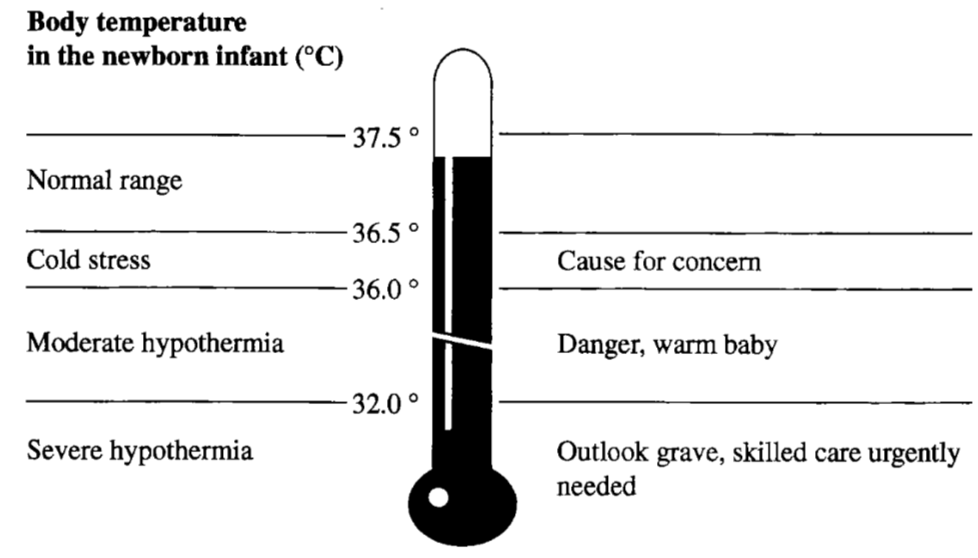
\includegraphics[width=350pt,height=200pt]{images/clipboard-2554530258.png} % Adjust the path to your image
  \caption{Effective thermal protection for newborns is crucial, as hypothermia can occur rapidly post-delivery.}
  \label{fig:fig3}
\end{figure}

Effective management includes assessing for infections and implementing
safe heating practices to avoid burns. Conversely, hyperthermia, defined
as a body temperature exceeding 37.5°C, can result in dehydration and
necessitates quick evaluation for infections. Guidelines for incubator
use specify maintaining an air temperature of 35--36°C, conducting
regular temperature checks, ensuring cleanliness, and encouraging
skin-to-skin contact between newborns and their mothers. {[}1{]}

The MQTT protocol has been evaluated in both the biomedical engineering
laboratory and the hospital's neonatology unit. Premature infants often
lack sufficient body fat and organ development to maintain their body
temperature, which should be kept between 28°C and 34°C. Reducing access
time to newborns is vital to minimize heat and oxygen loss. {[}5{]}

The BreathAnalyzer, a smartwatch that uses an AI model based on decision
trees, improves accuracy in detecting respiratory sinus arrhythmia (RSA)
from 35.37\% to 80\%, achieving an average of 42\% accuracy across
various scenarios. Calibration tests were conducted in accordance with
the ISO/IEC 1725:2017 standard to ensure measurement reliability.
Despite advancements, there are no existing devices that fully meet the
needs of the medical field. The Internet of Things in medicine (IoMT) is
essential for developing comprehensive technological solutions. However,
a progressive web application (SiMCa-Bio) was created to monitor
incubator conditions in real-time, focusing only on temperature,
humidity, and sound, with a sampling frequency of 5 minutes and data
transmission every 10 minutes {[}5{]}. Hoever Elevated levels of
relative humidity are not advisable for infants, as they can encourage
the growth of bacteria and germs {[}6{]}

The transition from traditional monitoring methods to wearable devices
focuses on reducing adhesive-related skin injuries. This approach
promotes the use of soft, flexible materials and gentler adhesion
techniques while emphasizing the design of all-in-one devices. The
priority is on non-invasive monitoring solutions that enhance
accessibility, particularly for high-risk patients, such as those born
prematurely (with a gestational age of less than 37 weeks) or with low
birth weight (typically less than 2.5 kg) {[}7{]}

Smart infant incubator monitoring and control system that utilizes a gas
sensor, accelerometer, and Peltier module, which are not part of our
current design was developed by K C N Raju {[}8{]}. The system
automatically adjusts the Peltier module and humidifier when
temperatures exceed 36°C to 37.2°C and humidity exceeds 60\%, ensuring
an optimal environment for premature and critically ill newborns.

A major challenge identified is the imbalance between caregivers and
patients, leading to increased workloads and compromised monitoring of
incubators. The study emphasizes maintaining temperatures between 36°C
and 37.5°C, with a targeted rectal temperature of around 36°C, and
humidity levels between 40\% and 60\%. Additionally, the integration of
artificial intelligence and live monitoring through cameras enhances the
care provided. However, limitations include the use of an Arduino Wi-Fi
R3 and reliance on an LCD display and ThingSpeak for IoT applications.

Another study {[}9{]} focuses on an IoT-based baby incubator monitoring
system utilizing Raspberry Pi Zero W. It monitors critical environmental
parameters, including temperature, humidity, and oxygen levels, in
real-time to safeguard infants in incubators. The system is connected to
a central computer for data visualization, alarms, and alerts, enabling
healthcare professionals to monitor the situation remotely. The
incubator is maintained at a temperature range of 32 to 36 degrees
Celsius to ensure the baby's skin remains at a healthy temperature of 37
degrees Celsius. Additionally, appropriate humidity levels warm the
baby's breath and facilitate the entry of moist air into the lungs.

Adding on to it, {[}10{]} emphasized that heating systems require
careful management, particularly during the winter months, to maintain a
consistent temperature for optimal comfort. Humidity levels in solids
and liquids are measured using hygrometers. Various methods for
measuring moisture include assessing changes in resistivity, variations
in capacitance, or monitoring the attenuation of microwaves.

This literature {[}10{]} provided information regarding checksum
{[}11{]} for a typical DHT22 sensor that was in communication via I2C
protocol:

\[ 
Data Structure = 8 bits (RH_{int}) + 8 bits (RH_{dec}) + 8 bits (T_{int}) + 8 bits (T_{dec}) + 8 Checksum Bits 
\]

Where, \(RH_{int}\) = Integer Relative Humidity, \(RH_{dec}\) = Decimal
Relative Humidity, \(T_{int}\) = Integer Temperature and \(T_{dec}\) =
Decimal Temperature.

Around 75,000 children worldwide suffer from brain dysfunction due to
jaundice, with neonatal hyperbilirubinemia causing approximately 114,100
preventable deaths and many long-term disabilities. Transcutaneous
Bilirubin (TcB) is a non-invasive method for jaundice detection, with
its phototherapy roots tracing back to England, where sunlight exposure
was linked to reduced jaundice in infants. Bilirubin absorbs light
predominantly in the blue spectrum near 460 nm, triggering photochemical
reactions in the skin. The most effective treatment involves light in
the 460 to 490 nm range. In this study, a camera was set 30 cm from the
subject at a 45-degree angle under 200 lux ambient lighting, using color
transformation and Otsu thresholding for skin detection. {[}12{]}

A limitation of this approach is the dependence on MATLAB, a commercial
software, which lacks on-device detection capabilities.

The study examines neonatal hyperbilirubinemia and Rhesus disease,
focusing on their incidence and impacts in 2010. It highlights the
critical importance of early detection and effective management to
prevent severe outcomes, such as neurological damage and mortality. The
authors urge health systems to prioritize these strategies to reduce
morbidity and mortality rates. Key takeaways include the necessity of
early detection, the potential of treatment protocols to mitigate
long-term impairments, and the benefits of incorporating screening
methods to enhance neonatal health outcomes. {[}13{]}

\section{Objectives}\label{objectives}

\subsection{Primary Objectives}\label{primary-objectives}

\begin{enumerate}
\def\labelenumi{\arabic{enumi}.}
\item
  \textbf{Affordablity}: Develop a low-cost yet cutting-edge device that
  enhances healthcare delivery in resource-limited settings, ensuring
  accessibility for all.
\item
  \textbf{Real-Time Monitoring of Essential Health Metrics}: Implement
  continuous monitoring capabilities for vital health parameters that
  includes body temperature {[}14{]}, ambient temperature, ambient
  humidity levels, neonatal heart rate, blood oxygen saturation
  (\(SpO_2\)) and Electrocardiogram (ECG).
\item
  \textbf{User-Friendly Touch Screen Interface}: Design an intuitive
  touch-screen user interface that simplifies interaction with the
  device.
\item
  \textbf{Comprehensive Data Logging}: Facilitate automatic logging of
  health data over time, enabling caregivers to track trends and make
  informed decisions regarding the care of premature newborns.
\item
  \textbf{Remote Data Accessibility via IoT}: Enable remote access to
  device data through IoT integration, allowing healthcare professionals
  to monitor patients' conditions from distant locations, enhancing
  collaboration and response times.
\item
  \textbf{Critical Alarm System}: Integrate a robust alarm system that
  alerts caregivers to critical changes in health parameters, ensuring
  prompt action can be taken in emergencies.
\item
  \textbf{Phototherapy Capabilities}: Include a phototherapy function
  for the treatment of neonatal jaundice, utilizing advanced light
  therapy to support the health and recovery of affected infants.
\end{enumerate}

\subsection{Secondary Objectives}\label{secondary-objectives}

\begin{enumerate}
\def\labelenumi{\arabic{enumi}.}
\item
  \textbf{AI-Driven Jaundice Detection and Classification}: Explore the
  potential for AI integration to enhance jaundice detection and
  classification {[}12{]} based on Kramer's rule. Availability of data
  is the major problem to implement this. A potential dataset {[}15{]}
  was found that can help us meet this objective.
\item
  \textbf{Produce Instantaneous Reports}: Create a reporting function
  that generates up-to-date health status reports, enabling healthcare
  professionals to swiftly evaluate the condition of premature infants
  without the need for manual data input.
\item
  \textbf{Compliance and Record Keeping}: Establish automated reporting
  that aligns with healthcare standards and regulations, simplifying the
  record-keeping process for neonatal care and ensuring accessibility
  for audits and assessments.
\end{enumerate}

\section{Materials and Methods}\label{materials-and-methods}

\subsection{Materials}\label{materials}

\subsubsection{Software requirements}\label{software-requirements}

Software used is listed in the table \ref{tab:table1}

\begin{table}[h]
    \centering
    \caption{Software Requirements for Project}
    \begin{tabular}{@{}lll p{1cm} p{4cm}@{}}
        \toprule
        \textbf{Software} & \textbf{Inventor/Developer} & \textbf{Open Source / Paid} & \textbf{Version} & \textbf{Purpose} \\
        \midrule
        KiCAD & Jean-Pierre Charras & Open Source & 7.0.0 & Schematic and PCB design \\
        Python & Python Software Foundation & Open Source & 3.12.0 & Programming \\
        Thonny & Aivar Annamaa & Open Source & 4.1.1 & Microcontroller firmware \\
        Visual Studio Code & Microsoft & Open Source & 1.82.0 & Code editing, debugging \\
        Node RED & JS Foundation (IBM) & Open Source & 3.1.0 & IoT workflows automation \\
        Grafana & Grafana Labs & Open Source & 10.1.1 & Data visualization \\
        Influx DB & InfluxData & Open Source & 2.7.0 & Time-series database \\
        HTML, CSS, JavaScript & Various & Open Source & - & Web Development \\
        PyQt5 & Riverbank Computing & Open Source (GPL) & 5.15.9 & On Device GUI \\
        MySQL & Oracle Corporation & Open Source (GPL) & 8.1.0 & DBMS \\
        \bottomrule
    \end{tabular}
    \label{tab:table1}
\end{table}

\subsubsection{Hardware requirements}\label{hardware-requirements}

Refer Table \ref{tab:table2} given below for hardware components used in
the project.

\begin{table}[h]
    \centering
    \caption{Hardware Requirements}
    \begin{tabular}{@{}lllp{2cm}@{}}
        \toprule
        \textbf{Item No.} & \textbf{Part Description} & \textbf{Specs} & \textbf{Quantity} \\
        \midrule
        1 & Non Contact Temperature Sensor & MLX90614 ESF & 1 \\
        2 & Temperature and Relative Humidity Sensor & GY-SHT40 & 1 \\
        3 & SpO2 and Heart Rate Sensor & MAX30102 & 1 \\
        4 & Sound Sensor & MAX9814 & 1 \\
        5 & ECG Module + Cables + Electrodes & AD8232 & 1 \\
        6 & Microcontroller board & RP2350 Pico 2 board & 1 \\
        7 & Ambient Light sensor for Phototherapy Unit & VEML6030 & 1 \\
        8 & ECG Gel Electrodes & 3 each in 5 Packs & 2 \\
        9 & Raspberry Pi Memory Card & Raspberry Pi Official 32GB V3.0, A2 Class & 1 \\
        10 & Raspberry Pi Microprocessor Board & Raspberry Pi 5 Model B 8GB RAM & 1 \\
        11 & Active Cooler for Microprocessor Board & - & 1 \\
        12 & Raspberry Pi Power Supply & 27W USB-C PD Power Supply & 1 \\
        13 & IO Expansion Hat for RPI 5 & - & 1 \\
        14 & Micro HDMI to HDMI Cable & Official RPi 5 Micro HDMI to HDMI & 1 \\
        15 & SpO2 Probe & - & 1 \\
        16 & RS232 to USB Adapter for SpO2 Probe & - & 1 \\
        17 & ASAIR AO-08 Medical Oxygen Sensor & ASAIR AO-08 & 1 \\
        18 & RPI Camera Module 3 NoIR – Wide & Sony IMX706 & 1 \\
        19 & Ultrasonic Humidifier & - & 1 \\
        20 & PTC Heating element & - & 1 \\
        \bottomrule
    \end{tabular}
    \label{tab:table2}
\end{table}

\subsection{Methods}\label{methods}

Tentative workflow for the project is given in figure \ref{fig:fig4}

\begin{figure}
  \centering
  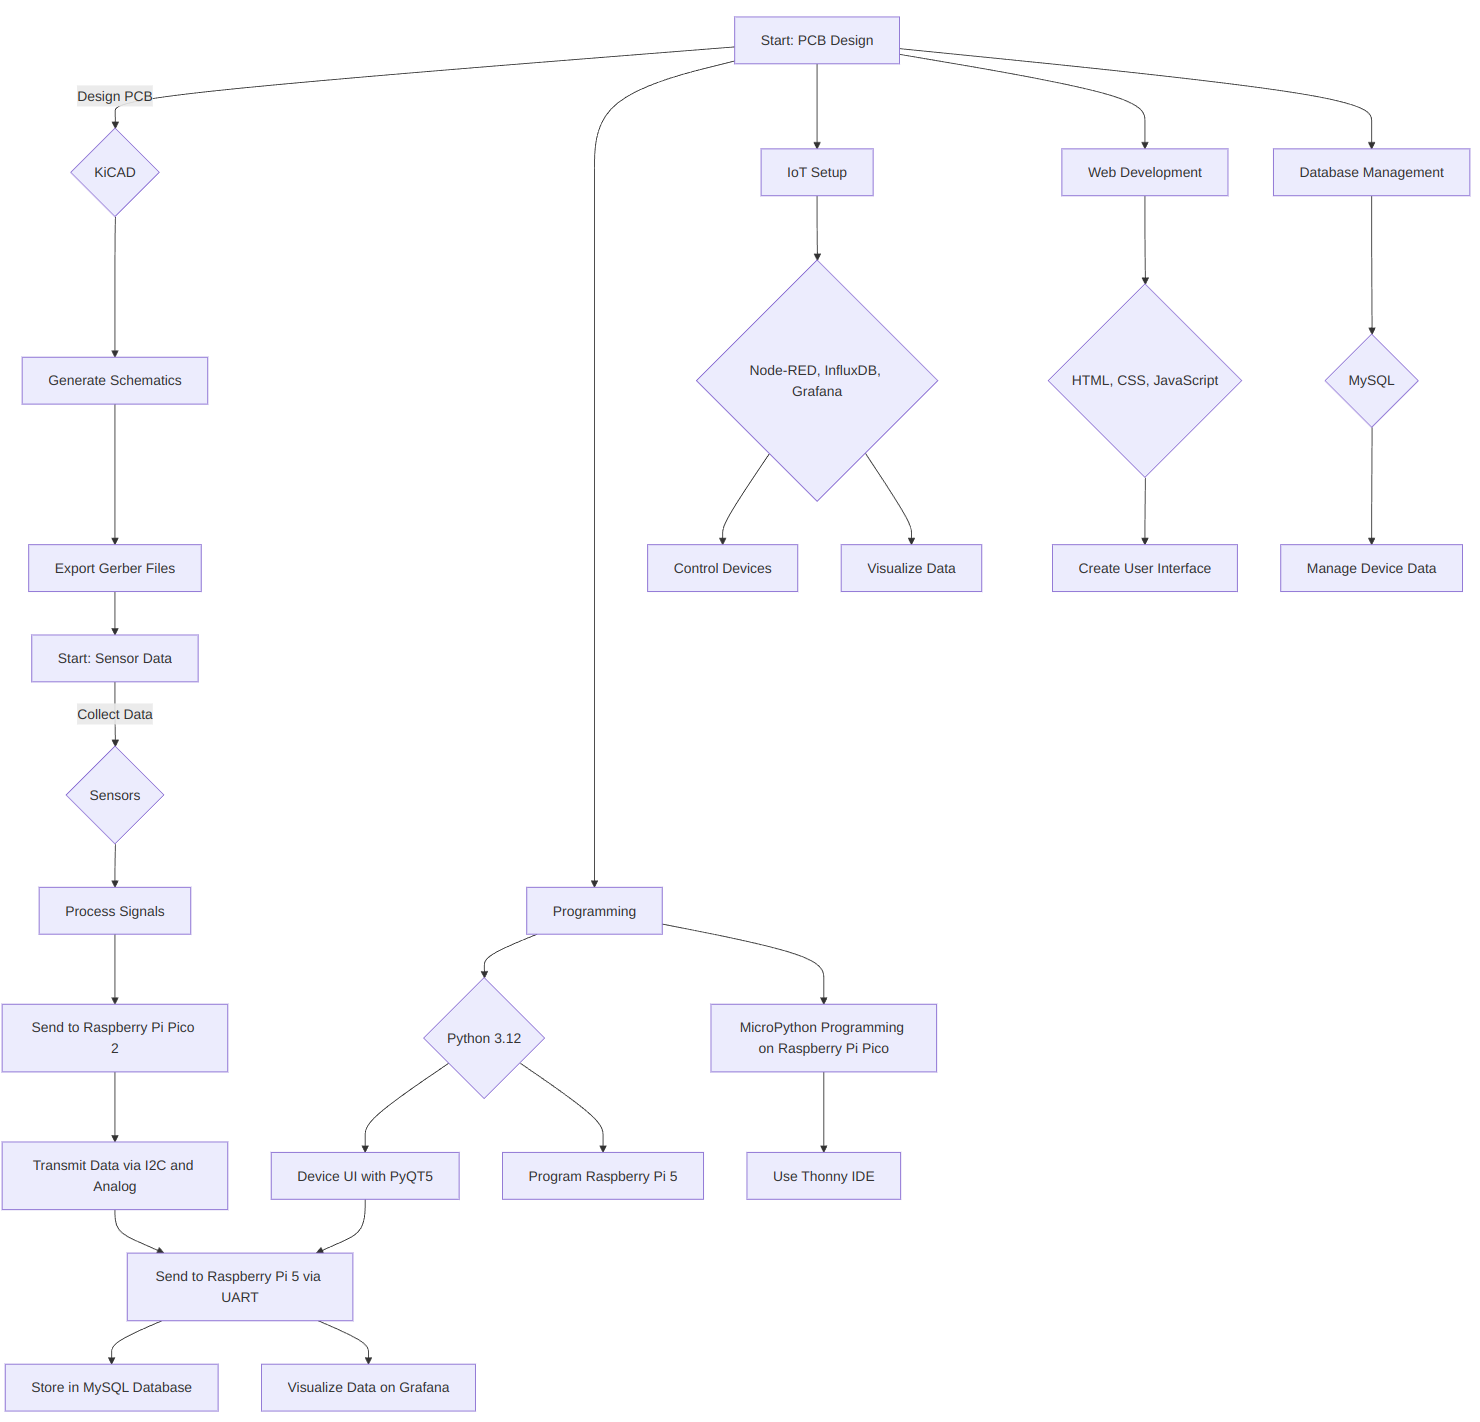
\includegraphics[width=500pt,height=500pt]{images/clipboard-1005866267.png} % Adjust the path to your image
  \caption{Key stages and processes involved in developing the project. `}
  \label{fig:fig4}
\end{figure}

\subsubsection{Why does this methodology
work?}\label{why-does-this-methodology-work}

The workflow method applied in this project from PCB design to data
visualization. Each stage is interconnected, promoting efficient data
processing and communication between devices.

\begin{enumerate}
\def\labelenumi{\arabic{enumi}.}
\tightlist
\item
  \textbf{PCB Design:} The use of KiCAD {[}16{]} for PCB design allows
  for precise generation of schematics and layouts. This structured
  approach ensures that the hardware is optimally configured for
  subsequent processes. {[}17{]}. See figure \ref{fig:fig5} for
  schematic and figure \ref{fig:fig6} for layout design
\end{enumerate}

\begin{figure}
  \centering
  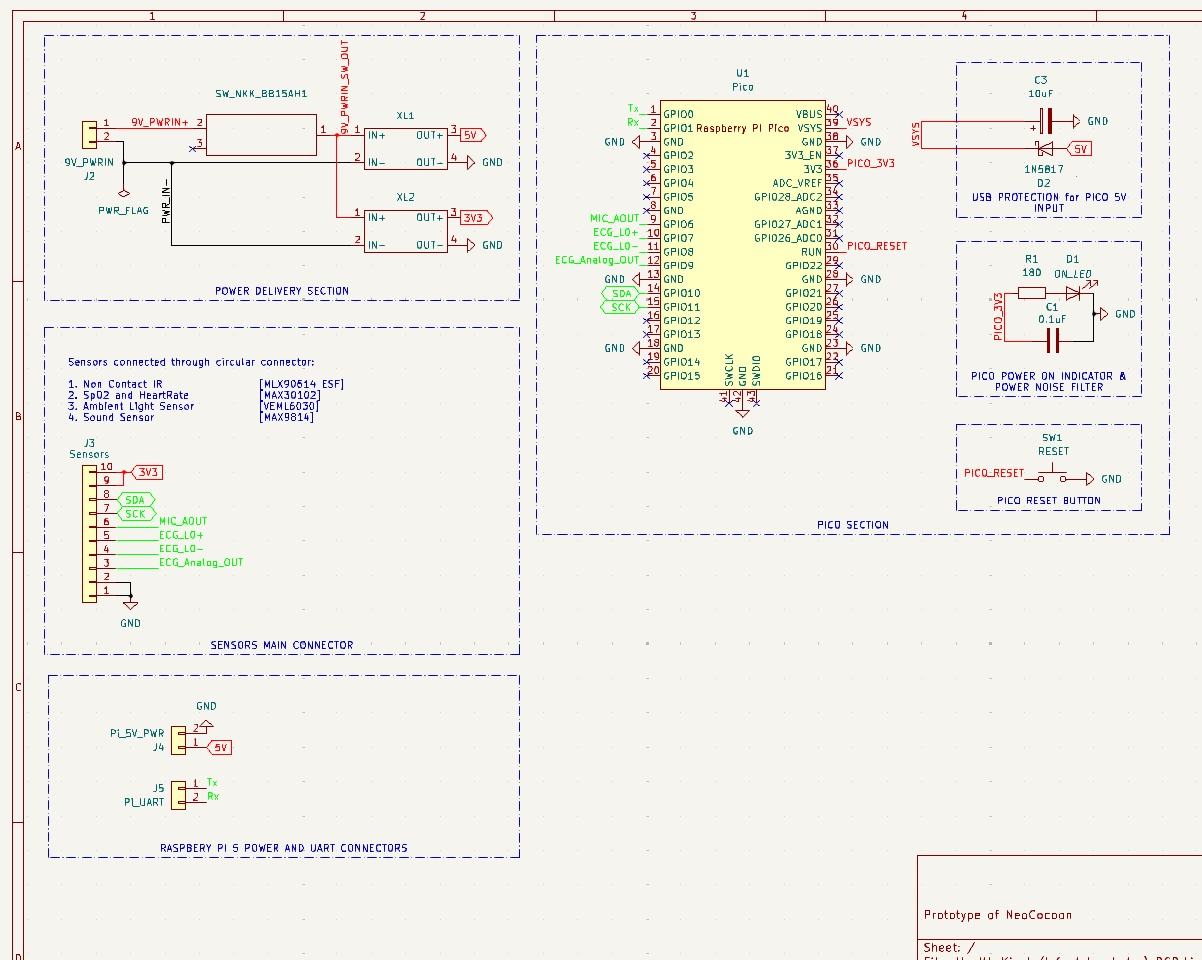
\includegraphics[width=300pt,height=250pt]{images/schematic.jpeg} % Adjust the path to your image
  \caption{Schematic containing circuits seperated as different sections for enhancing readability.}
  \label{fig:fig5}
\end{figure}

\begin{figure}
  \centering
  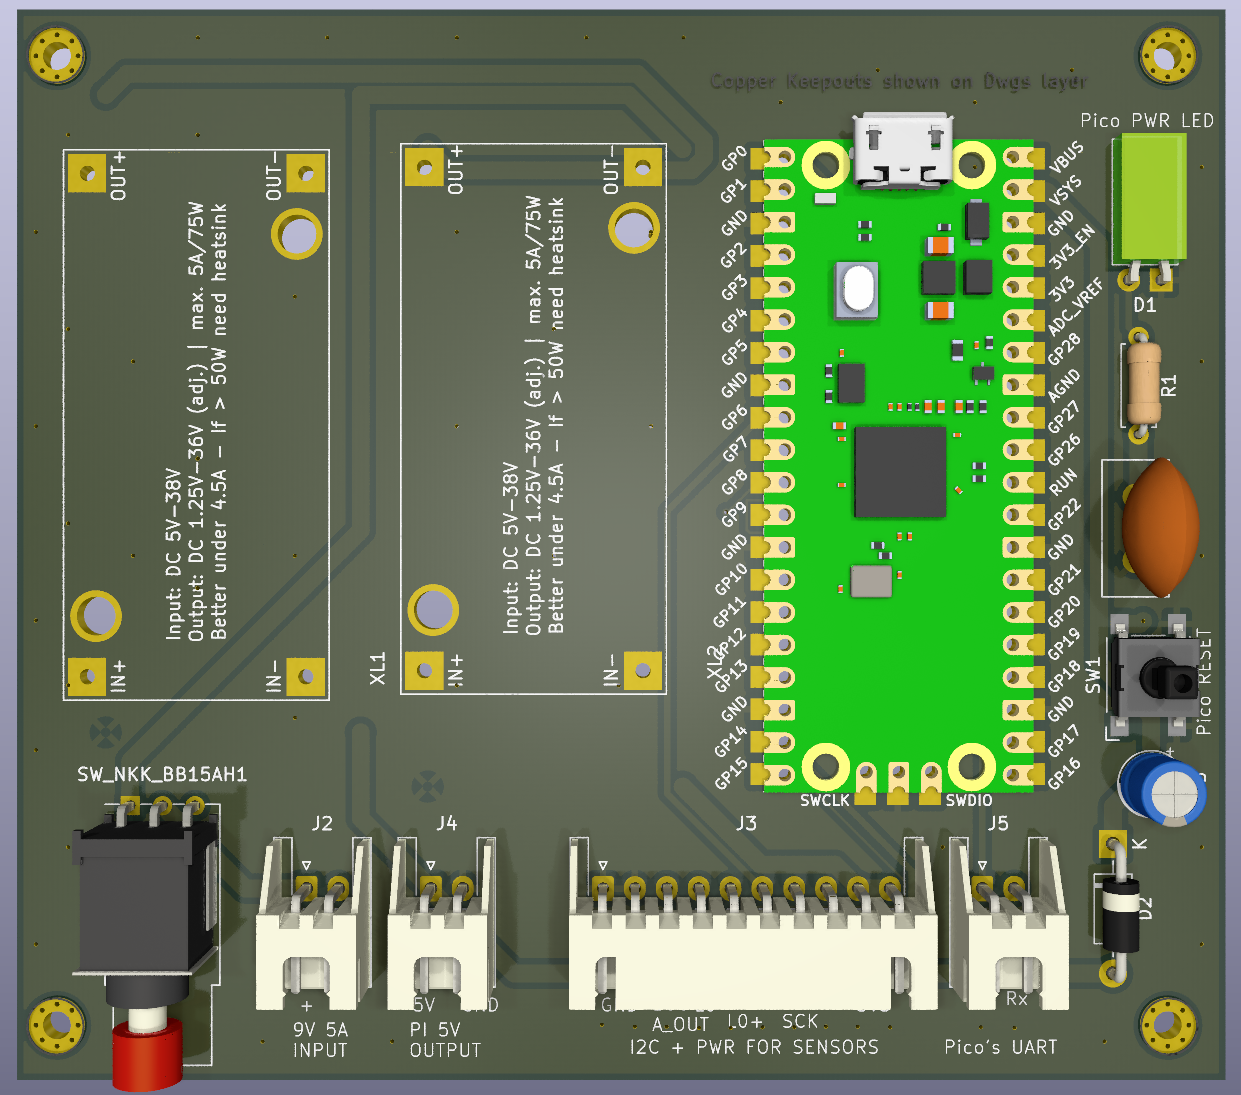
\includegraphics[width=300pt,height=280pt]{images/pcb.png} % Adjust the path to your image
  \caption{PCB incorporating power delivery, communication, connectors, microcontroller reset button and power noise filter.}
  \label{fig:fig6}
\end{figure}

\begin{enumerate}
\def\labelenumi{\arabic{enumi}.}
\setcounter{enumi}{1}
\item
  \textbf{Microcontroller Programming:} The workflow effectively
  leverages the capabilities of the Raspberry Pi Pico 2 through
  MicroPython, programmed using Thonny. This combination allows for
  direct hardware manipulation, essential for handling sensor data
  collection accurately. The I2C and Analog interfaces used for data
  transmission enable effective communication between the sensors and
  the microcontroller.
\item
  \textbf{Microprocessor Programming:} Implementing Python 3.12 on the
  Raspberry Pi 5 facilitates a robust programming environment for
  developing the device's user interface (See figure \ref{fig:fig7} and
  figure \ref{fig:fig8}). Python's extensive libraries simplify complex
  programming tasks, making it an ideal choice for creating responsive
  and interactive applications.
\item
  \textbf{Data Transmission Protocols:} Sensor data is communicated
  through I2C and Analog. The transmission of raw data from the
  Raspberry Pi Pico 2 to the Raspberry Pi 5 via UART ensures that data
  is transferred swiftly and reliably.
\item
  \textbf{IoT Integration:} The integration of Node-RED, InfluxDB, and
  Grafana into the workflow enhances the Internet of Things (IoT)
  capabilities of the project. Node-RED facilitates flow-based
  programming, allowing users to design workflows visually, while
  InfluxDB stores time-series data efficiently. Grafana then visualizes
  this data, providing insightful dashboards for users to monitor and
  analyze system performance.
\item
  \textbf{Database Management:} Utilizing MySQL for database management
  {[}18{]} establishes a reliable repository for storing device data.
  This approach to data organization ensures that information can be
  retrieved quickly.
\end{enumerate}

\begin{figure}
  \centering
  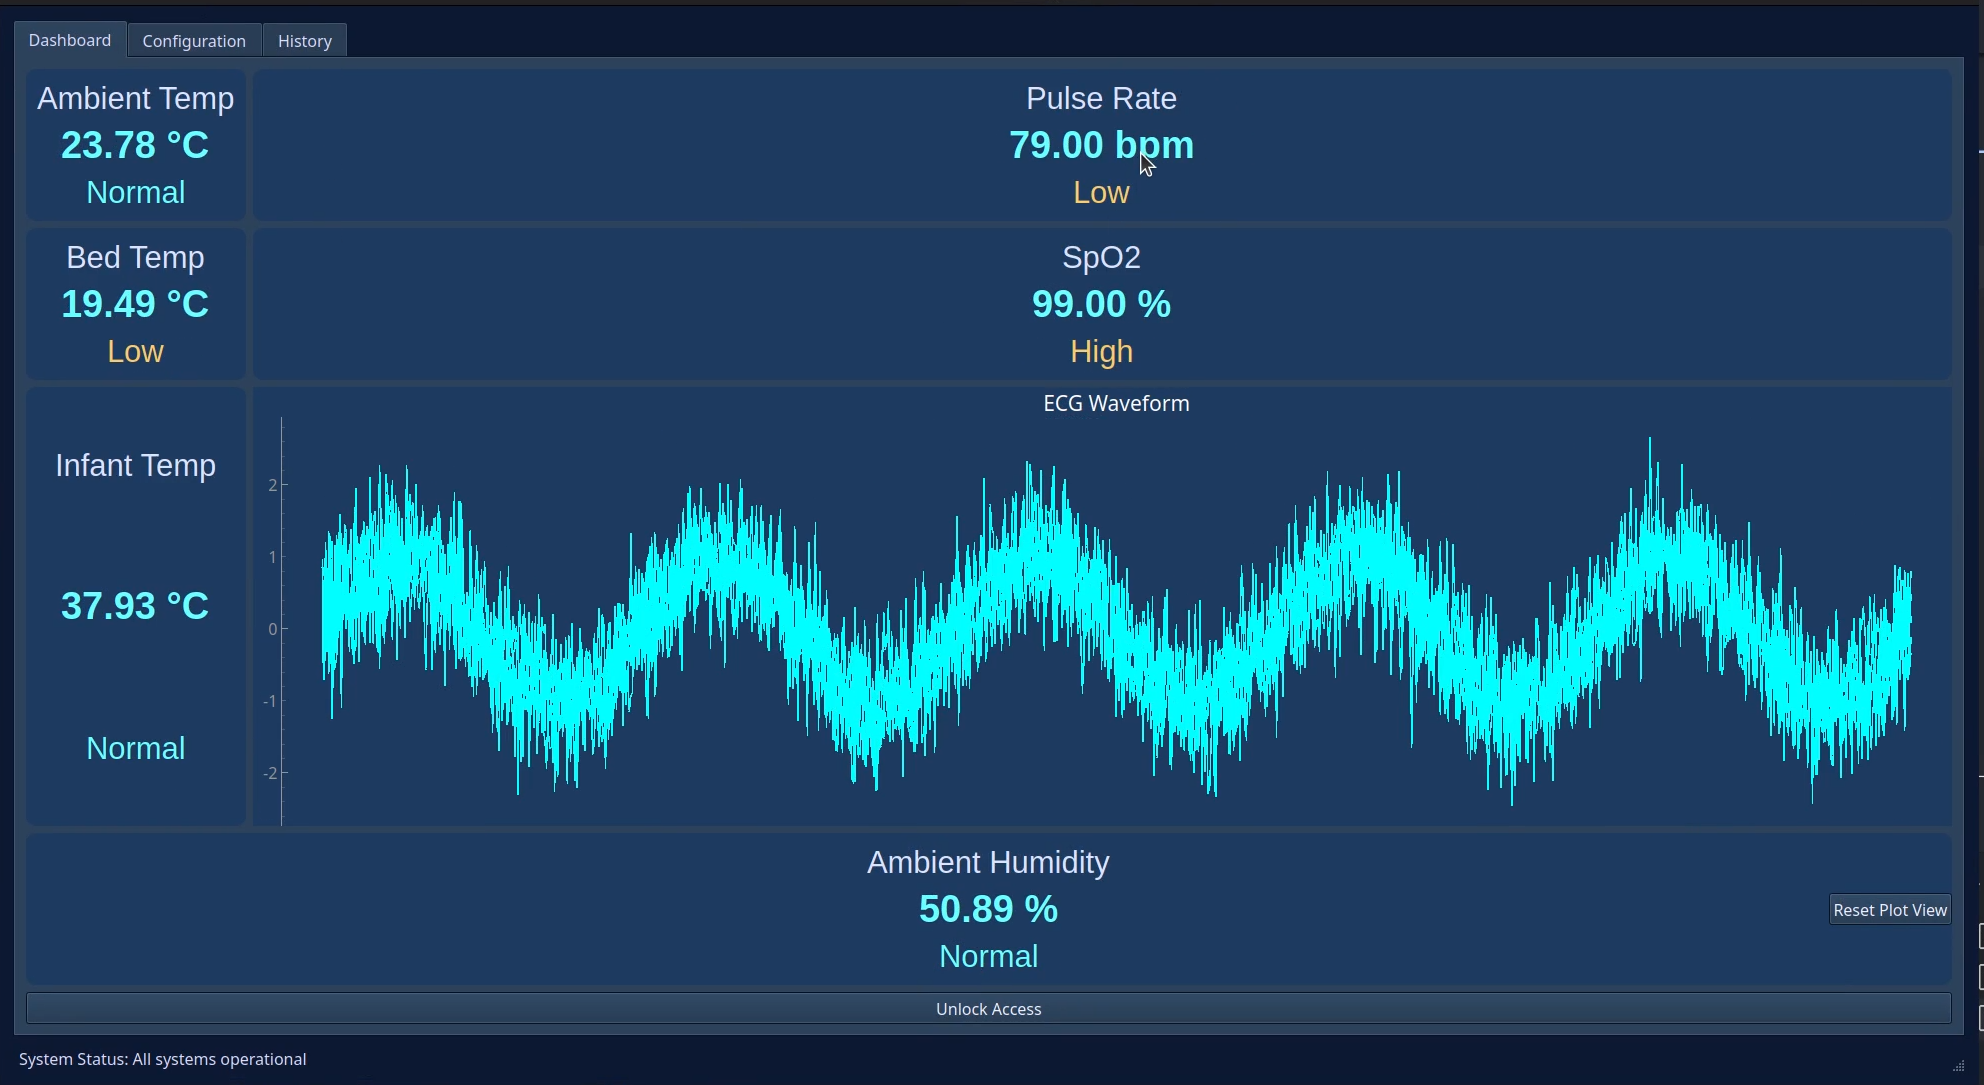
\includegraphics[width=450pt,height=280pt]{images/ui1.png} % Adjust the path to your image
  \caption{Touch screen based Main Graphical user Interface shwowing vital health parameters for quick look and easy interaction.}
  \label{fig:fig7}
\end{figure}

\begin{figure}
  \centering
  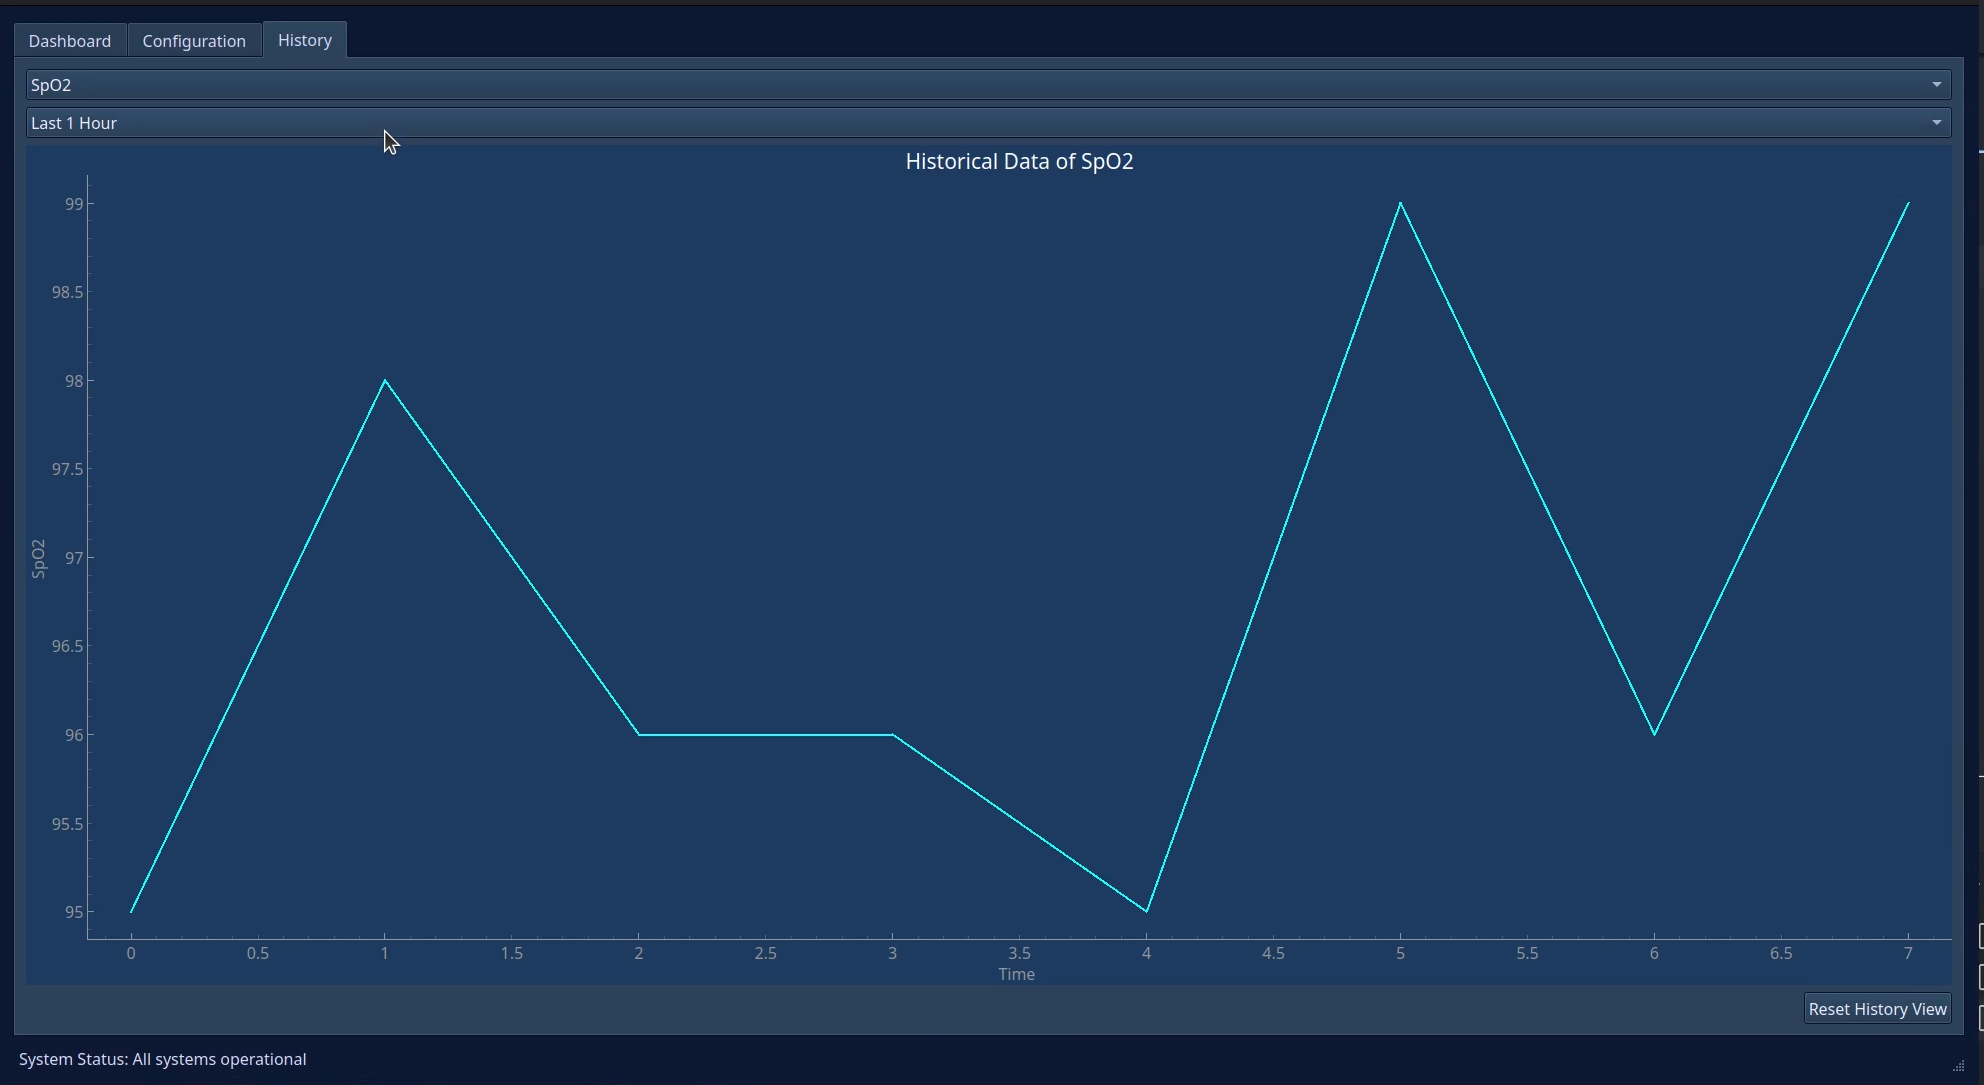
\includegraphics[width=450pt,height=260pt]{images/ui2.png} % Adjust the path to your image
  \caption{GUI based History access for more insights during realtime monitoring.}
  \label{fig:fig8}
\end{figure}

\paragraph{Paying attention to Non Contact Infrared Temperature (NCIT)
Measurement}\label{paying-attention-to-non-contact-infrared-temperature-ncit-measurement}

This study {[}19{]} focuses on utilizing an infrared human body
temperature sensor to convert the body's infrared radiation into a
voltage signal. Experimental results indicate a temperature measurement
error of less than 0.2°C, with a measurement time of approximately 4
seconds using a non-contact infrared thermometer. In contrast, mercury
thermometers require direct contact and can take 5 to 10 minutes to
measure temperature, often leading to inaccuracies due to external light
interference.

The principle of infrared temperature measurement is based on the
emission of electromagnetic waves from objects with temperatures above
absolute zero, with the intensity of radiation depending on the object's
absolute temperature. Notably, all real objects, including the human
body, have Beta values less than 1.0, and the main infrared radiation
wavelength of the human body ranges from 9 to 10 um. This wavelength is
not absorbed by air, allowing for accurate surface temperature
determination based on infrared energy. {[}19{]}

This literature {[}20{]} critically examines the performance of
non-contact infrared thermometers (NCITs) and infrared thermometers
(IRT) in monitoring body temperature, synthesizing data from 72 unique
settings across 32 studies. Both NCITs and IRTs showed a positive
correlation with traditional contact-based temperature measurement
tools; however, NCITs exhibited slightly greater accuracy. Specifically,
29 out of 50 settings from NCIT studies and 4 out of 22 settings from
IRT studies achieved accuracy levels within ±0.3°C. This suggests that
while both types of thermometers are effective, NCITs may be the
preferable option for more precise temperature monitoring.

\paragraph{Do NCITs have edge over traditional contact based temperature
measurement?}\label{do-ncits-have-edge-over-traditional-contact-based-temperature-measurement}

Traditional methods of measuring body temperature often involve affixing
sensors directly to the skin, which can compromise measurement accuracy
due to environmental disturbances. A review that included 21 studies
revealed that the bias in temperature readings can vary widely; some
setups demonstrated minor discrepancies of less than 0.5°C, while others
exhibited significant errors exceeding 0.5°C. These findings highlight
the considerable influence that setup variables have on the accuracy of
contact-based temperature sensors. Therefore, consistent documentation
of these variables across studies is essential for accurate
interpretation and reliable comparisons among different research
findings. {[}21{]}

\paragraph{Deciding between Resistive and Capacitive Touch Screen
technologies in healthcare
setting}\label{deciding-between-resistive-and-capacitive-touch-screen-technologies-in-healthcare-setting}

\begin{table}[h]
    \centering
    \caption{Comparison of Resistive and Capacitive Touchscreens}
    \begin{tabular}{@{}lll@{}}
        \toprule
        Feature                  & Resistive Touchscreen                      & Capacitive Touchscreen                     \\ \midrule
        Structure                & Multiple layers with a conductive gap      & Single insulating layer with conductive film \\ 
        Interaction Method       & Detects pressure                           & Detects change in electric field           \\
        Input Types              & Any touch (conductive or non-conductive)  & Only conductive touch (e.g., human finger)  \\
        Accuracy                 & Moderate                                  & High                                      \\
        Response Time            & Slower                                    & Faster                                    \\ 
        Applications             & Versatile (various objects)               & Preferred for precise touch input          \\ \bottomrule
    \end{tabular}
\end{table}

While resistive touchscreens can register touch from various objects,
capacitive touchscreens are more efficient and responsive, making them a
preferred choice for applications requiring precise touch input, hence
we choose this technology.

\section{Expected Outcomes}\label{expected-outcomes}

\begin{itemize}
\item
  \textbf{Improved Public Health Monitoring}

  The development of a non-contact infrared temperature measurement
  system will enhance early detection of fever, a common indicator of
  infection, allowing for timely intervention and reducing the spread of
  infectious diseases.
\item
  \textbf{Accessibility and Convenience}

  The non-invasive nature of the device makes it suitable for use in
  diverse settings, including homes, schools, and healthcare facilities,
  thereby increasing accessibility to health monitoring tools,
  particularly in resource-limited environments. Reduction of
\item
  \textbf{Healthcare Costs}

  By facilitating early detection and monitoring of health conditions,
  the technology can potentially lower healthcare costs associated with
  hospital visits and treatments for advanced-stage illnesses.
\item
  \textbf{Enhanced Safety in Healthcare Settings}

  The ability to measure temperature without physical contact reduces
  the risk of cross-contamination, thus enhancing safety protocols in
  hospitals and clinics, especially in the context of infectious disease
  outbreaks.
\item
  \textbf{Support for Pediatric Care}

  The technology is particularly beneficial for monitoring infants and
  young children, providing parents and caregivers with a safe and
  efficient method for tracking body temperature without causing
  discomfort.
\item
  \textbf{Contribution to Research and Development}

  The insights gained from the implementation and performance evaluation
  of the system can contribute to the broader field of biomedical
  engineering and health technology research, fostering innovation and
  encouraging further advancements.
\item
  \textbf{Potential for Integration with Smart Health Systems}

  The device can be integrated into existing health monitoring systems
  and IoT platforms, paving the way for advanced health analytics and
  real-time data sharing, which can enhance public health responses
  during emergencies.
\end{itemize}

\section{Grants}\label{grants}

We would like to extend my sincere gratitude to the \textbf{MSME
Government of India} for their generous funding and support for this
project. Their commitment to fostering innovation and entrepreneurship
has been instrumental in making this initiative possible.

\section{Acknowledgement}\label{acknowledgement}

We would like to express our gratitude and sincere thanks to our
internal guide Dr.~H N Suma and external guide Mr.~Balaji Raghavendra S
for giving us the opportunity and providing complete guidance throughout
our project. Secondly, we would like to thank all the faculty members of
our department for being a supportive part in our learning process.
Further we would also like to thank our team members whose guidance,
encouragement and suggestions have contributed immensely to the
evolution of better ideas and completion of the project.

\newpage

\section{PO Attainment}\label{po-attainment}

\begin{table}[ht]
    \centering
    \caption{Program Outcomes (PO) and Program Specific Outcomes (PSO)}
    \begin{tabular}{@{}ll@{}}
        \toprule
        \textbf{Outcome Code} & \textbf{Description} \\ \midrule
        PO1  & \begin{minipage}[t]{10cm} \textbf{Engineering Knowledge:} Utilized engineering principles to design the hardware components neccessary and know-how of software aspects of the projet. Plan is done to implement the designs. \end{minipage} \\
        PO2  & \begin{minipage}[t]{10cm} \textbf{Problem Analysis:} Identified challenges in care of pre mature newborns, risks and consequences associated with it. \end{minipage} \\
        PO3  & \begin{minipage}[t]{10cm} \textbf{Design/Development of Solutions:} Ongoing design for an innovative temperature monitoring system that incorporates advanced sensing technologies and reliable communication protocols. \end{minipage} \\
        PO4  & \begin{minipage}[t]{10cm} \textbf{Conduct Investigation of Complex Problems:} Conducted thorough investigations into the effectiveness of different sensor technologies with acceptable error margins for healthcare settings. \end{minipage} \\
        PO5  & \begin{minipage}[t]{10cm} \textbf{Modern Tool Usage:} Leveraged modern tools like KiCAD for PCB design, Python and IoT for software development in conjuction with hardware. \end{minipage} \\
        PO6  & \begin{minipage}[t]{10cm} \textbf{Engineer and Society:} Developing a solution that addresses neonatal health issues, contributing positively to society. \end{minipage} \\
        PO7  & \begin{minipage}[t]{10cm} \textbf{Environment and Sustainability:} Ensured the design is energy-efficient and minimizes waste in manufacturing processes. \end{minipage} \\
        PO8  & \begin{minipage}[t]{10cm} \textbf{Ethics:} Adhered to ethical guidelines in medical device development, prioritizing patient safety and listed out medical standards neccessary to be met. \end{minipage} \\
        PO9  & \begin{minipage}[t]{10cm} \textbf{Individual and Teamwork:} Collaborated with team to achieve project goals while also managing individual tasks. \end{minipage} \\
        PO10 & \begin{minipage}[t]{10cm} \textbf{Communication:} Effectively communicated complex concepts and findings to MSME Govt of India when they had visited for signing funds in both technical and non-technical aspects. \end{minipage} \\
        PO11 & \begin{minipage}[t]{10cm} \textbf{Project Management:} Managing project timelines and resources efficiently, ensuring successful delivery of project milestones. \end{minipage} \\
        PO12 & \begin{minipage}[t]{10cm} \textbf{Life-Long Learning:} Engaged in continuous learning to stay updated with emerging technologies in biomedical engineering. \end{minipage} \\ \midrule
        PSO1 & \begin{minipage}[t]{10cm}\textbf{ Investigate, Implement, and Demonstrate biomedical systems:} To be done in the upcoming weeks \end{minipage} \\
        PSO2 & \begin{minipage}[t]{10cm} \textbf{Specify, Architect, and Prototype healthcare solutions:} Prototyping a healthcare solution that utilizes new technolgies such as infrared technology for non-contact temperature measurement. \end{minipage} \\
        PSO3 & \begin{minipage}[t]{10cm} \textbf{Design, Develop, and Verify algorithms for medical purposes:} Developing algorithms for accurate temperature detection and verification using sensor data. \end{minipage} \\ \bottomrule
    \end{tabular}
    \label{tab:outcomes}
\end{table}

\section*{References}\label{references}
\addcontentsline{toc}{section}{References}

\phantomsection\label{refs}
\begin{CSLReferences}{0}{0}
\bibitem[\citeproctext]{ref-noauthor_thermal_nodate}
\CSLLeftMargin{{[}1{]} }%
\CSLRightInline{{``Thermal protection of the newborn: A practical
guide.''} Accessed: Oct. 19, 2024. {[}Online{]}. Available:
\url{https://www.who.int/publications/i/item/WHO_RHT_MSM_97.2}}

\bibitem[\citeproctext]{ref-noauthor_low_nodate}
\CSLLeftMargin{{[}2{]} }%
\CSLRightInline{{``Low {Birth} {Weight}.''} Accessed: Oct. 19, 2024.
{[}Online{]}. Available:
\url{https://www.stanfordchildrens.org/en/topic/default?id=low-birth-weight-90-P02382}}

\bibitem[\citeproctext]{ref-noauthor_nacimientos_nodate}
\CSLLeftMargin{{[}3{]} }%
\CSLRightInline{{``Nacimientos prematuros.''} Accessed: Oct. 19, 2024.
{[}Online{]}. Available:
\url{https://www.who.int/es/news-room/fact-sheets/detail/preterm-birth}}

\bibitem[\citeproctext]{ref-noauthor_mortalidad_nodate}
\CSLLeftMargin{{[}4{]} }%
\CSLRightInline{{``Mortalidad neonatal.''} Accessed: Oct. 19, 2024.
{[}Online{]}. Available:
\url{https://www.who.int/es/news-room/fact-sheets/detail/newborn-mortality}}

\bibitem[\citeproctext]{ref-aya-parra_monitoring_2023}
\CSLLeftMargin{{[}5{]} }%
\CSLRightInline{P. A. Aya-Parra, A. J. Rodriguez-Orjuela, V. R. Torres,
N. P. C. Hernandez, N. M. Castellanos, and J. Sarmiento-Rojas,
{``Monitoring {System} for {Operating} {Variables} in {Incubators} in
the {Neonatology} {Service} of a {Highly} {Complex} {Hospital} through
the {Internet} of {Things} ({IoT}),''} \emph{Sensors (Basel,
Switzerland)}, vol. 23, no. 12, p. 5719, Jun. 2023, doi:
\href{https://doi.org/10.3390/s23125719}{10.3390/s23125719}.}

\bibitem[\citeproctext]{ref-pujiastuti_analysis_2022}
\CSLLeftMargin{{[}6{]} }%
\CSLRightInline{Y. Pujiastuti, A. Pudji, S. Y. Setiawan, F. Amrinsani,
and K. Phasinam, {``Analysis of {Temperature} {Stability} and {Accuracy}
on the {Design} of {Thermometer} {Calibrator} {Based} on {Fuzzy} {Logic}
{And} {On}/{Off} {Control},''} \emph{Journal of Electronics,
Electromedical Engineering, and Medical Informatics}, vol. 4, no. 3, pp.
144--153, Jul. 2022, doi:
\href{https://doi.org/10.35882/jeeemi.v4i3.244}{10.35882/jeeemi.v4i3.244}.}

\bibitem[\citeproctext]{ref-zhou_skin-interfacing_2024}
\CSLLeftMargin{{[}7{]} }%
\CSLRightInline{L. Zhou, M. Guess, K. R. Kim, and W.-H. Yeo,
{``Skin-interfacing wearable biosensors for smart health monitoring of
infants and neonates,''} \emph{Commun Mater}, vol. 5, no. 1, pp. 1--13,
May 2024, doi:
\href{https://doi.org/10.1038/s43246-024-00511-6}{10.1038/s43246-024-00511-6}.}

\bibitem[\citeproctext]{ref-k_c_n_smart_2024}
\CSLLeftMargin{{[}8{]} }%
\CSLRightInline{R. K C N, {``{SMART} {INFANT} {INCUBATOR} {MONITORING}
{AND} {CONTROL} {SYSTEM} {USING} {IoT},''} \emph{INTERNATIONAL JOURNAL
OF CREATIVE RESEARCH THOUGHTS}, vol. 12, pp. d786--d791, Mar. 2024.}

\bibitem[\citeproctext]{ref-ningsih_monitoring_2023}
\CSLLeftMargin{{[}9{]} }%
\CSLRightInline{F. Ningsih, B. Irianto, L. Lamidi, and M. Abdulhamid,
{``Monitoring {Baby} {Incubator} {Central} through {Internet} of
{Things} ({IoT}) based on {Raspberry} {Pi} {Zero} {W} with {Computer}
{Monitoring}),''} \emph{Indonesian Journal of Electronics,
Electromedical Engineering, and Medical Informatics}, vol. 5, pp.
116--124, Aug. 2023, doi:
\href{https://doi.org/10.35882/ijeeemi.v5i3.283}{10.35882/ijeeemi.v5i3.283}.}

\bibitem[\citeproctext]{ref-bogdan_sciendo_2016}
\CSLLeftMargin{{[}10{]} }%
\CSLRightInline{M. Bogdan, {``Sciendo,''} \emph{Acta Universitatis
Cibiniensis. Technical Series}, vol. 68, no. 1, pp. 22--25, Dec. 2016,
doi:
\href{https://doi.org/10.1515/aucts-2016-0005}{10.1515/aucts-2016-0005}.}

\bibitem[\citeproctext]{ref-maxino_effectiveness_2009}
\CSLLeftMargin{{[}11{]} }%
\CSLRightInline{T. C. Maxino and P. J. Koopman, {``The {Effectiveness}
of {Checksums} for {Embedded} {Control} {Networks},''} \emph{IEEE Trans.
Dependable and Secure Comput.}, vol. 6, no. 1, pp. 59--72, Jan. 2009,
doi:
\href{https://doi.org/10.1109/TDSC.2007.70216}{10.1109/TDSC.2007.70216}.}

\bibitem[\citeproctext]{ref-hashim_neonatal_2021}
\CSLLeftMargin{{[}12{]} }%
\CSLRightInline{W. Hashim, A. Al-Naji, I. A. Al-Rayahi, M. Alkhaled, and
J. Chahl, {``Neonatal {Jaundice} {Detection} {Using} a {Computer}
{Vision} {System},''} \emph{Designs}, vol. 5, no. 4, p. 63, Dec. 2021,
doi:
\href{https://doi.org/10.3390/designs5040063}{10.3390/designs5040063}.}

\bibitem[\citeproctext]{ref-bhutani_neonatal_2013}
\CSLLeftMargin{{[}13{]} }%
\CSLRightInline{V. K. Bhutani \emph{et al.}, {``Neonatal
hyperbilirubinemia and {Rhesus} disease of the newborn: Incidence and
impairment estimates for 2010 at regional and global levels,''}
\emph{Pediatric Research}, vol. 74, no. Suppl 1, p. 86, Dec. 2013, doi:
\href{https://doi.org/10.1038/pr.2013.208}{10.1038/pr.2013.208}.}

\bibitem[\citeproctext]{ref-wibawa_design_2022}
\CSLLeftMargin{{[}14{]} }%
\CSLRightInline{I. M. S. Wibawa and I. K. Putra, {``Design of air
temperature and humidity measurement based on {Arduino} {ATmega} {328P}
with {DHT22} sensor,''} \emph{International journal of physical sciences
and engineering}, vol. 6, no. 1, pp. 9--17, Jan. 2022, doi:
\href{https://doi.org/10.53730/ijpse.v6n1.3065}{10.53730/ijpse.v6n1.3065}.}

\bibitem[\citeproctext]{ref-abdulrazzak_njn_2023}
\CSLLeftMargin{{[}15{]} }%
\CSLRightInline{A. Y. Abdulrazzak, S. L. Mohammed, and A. Al-Naji,
{``{NJN}: {A} {Dataset} for the {Normal} and {Jaundiced} {Newborns},''}
\emph{BioMedInformatics}, vol. 3, no. 3, pp. 543--552, Sep. 2023, doi:
\href{https://doi.org/10.3390/biomedinformatics3030037}{10.3390/biomedinformatics3030037}.}

\bibitem[\citeproctext]{ref-noauthor_kicad_nodate}
\CSLLeftMargin{{[}16{]} }%
\CSLRightInline{{``{KiCad} {EDA}.''} Accessed: Oct. 19, 2024.
{[}Online{]}. Available: \url{https://www.kicad.org/}}

\bibitem[\citeproctext]{ref-noauthor_kicad_nodate-1}
\CSLLeftMargin{{[}17{]} }%
\CSLRightInline{{``{KiCad} - a tool for sharing, learning and developing
{\textbar} {CERN} \& {Society} {Foundation}.''} Accessed: Oct. 19, 2024.
{[}Online{]}. Available:
\url{https://cernandsocietyfoundation.cern/news/kicad-tool-sharing-learning-and-developing}}

\bibitem[\citeproctext]{ref-noauthor_mysql_nodate}
\CSLLeftMargin{{[}18{]} }%
\CSLRightInline{{``{MySQL} for the {Internet} of {Things} {\textbar}
{SpringerLink}.''} Accessed: Oct. 19, 2024. {[}Online{]}. Available:
\url{https://link.springer.com/book/10.1007/978-1-4842-1293-6}}

\bibitem[\citeproctext]{ref-long_sciendo_2016}
\CSLLeftMargin{{[}19{]} }%
\CSLRightInline{G. Long, {``Sciendo,''} \emph{International Journal on
Smart Sensing and Intelligent Systems}, vol. 9, no. 2, pp. 1110--1129,
Jun. 2016, doi:
\href{https://doi.org/10.21307/ijssis-2017-910}{10.21307/ijssis-2017-910}.}

\bibitem[\citeproctext]{ref-zhao_non-contact_2023}
\CSLLeftMargin{{[}20{]} }%
\CSLRightInline{Y. Zhao and J. H. M. Bergmann, {``Non-{Contact}
{Infrared} {Thermometers} and {Thermal} {Scanners} for {Human} {Body}
{Temperature} {Monitoring}: {A} {Systematic} {Review},''}
\emph{Sensors}, vol. 23, no. 17, p. 7439, Jan. 2023, doi:
\href{https://doi.org/10.3390/s23177439}{10.3390/s23177439}.}

\bibitem[\citeproctext]{ref-macrae_skin_2018}
\CSLLeftMargin{{[}21{]} }%
\CSLRightInline{B. A. MacRae, S. Annaheim, C. M. Spengler, and R. M.
Rossi, {``Skin {Temperature} {Measurement} {Using} {Contact}
{Thermometry}: {A} {Systematic} {Review} of {Setup} {Variables} and
{Their} {Effects} on {Measured} {Values},''} \emph{Front. Physiol.},
vol. 9, Jan. 2018, doi:
\href{https://doi.org/10.3389/fphys.2018.00029}{10.3389/fphys.2018.00029}.}

\end{CSLReferences}

\bibliographystyle{unsrt}
\bibliography{/home/karthik/NeoCocoon/Synopsis/Neococoon Zotero Export
Literature/Neococoon Zotero Export Literature.bib}


\end{document}
